\documentclass[11pt]{article}

\makeatletter
\newcommand{\skipitems}[1]{%
	\addtocounter{\@enumctr}{#1}%
}
\makeatother

\newcommand{\numpy}{{\tt numpy}}
\usepackage{amsfonts}
\usepackage{amsmath}
\usepackage{graphics}
\usepackage{amsthm,amstext,amsfonts,bm,amssymb}
\usepackage{graphicx}
\graphicspath{ {./images/} }
\usepackage{indentfirst}
\setlength{\parindent}{5ex}
\setlength{\parskip}{1em}
\usepackage[utf8x]{inputenc} 
\usepackage[russian]{babel}
\topmargin -.5in
\textheight 9in
\oddsidemargin -.25in
\evensidemargin -.25in
\textwidth 7in


\begin{document}
	
	\author{Биктимиров Данила, группа 204}
	\title{ДЗ 2}
	\date{}
	\maketitle
	
	\medskip
	
	\begin{enumerate}
		
		\item Рассмотрим последовательность $x_n = 1+\frac{1}{2}+...+\frac{1}{n} - \ln(n) $. Посмотрим на $\left\lvert x_{n+1} - x_n \right\rvert = \frac{1}{n+1} - \ln(\frac{n+1}{n}) = \frac{1}{n+1} - \frac{1}{n} + O(\frac{1}{n^2}) = \frac{1}{n(n+1)} + O(\frac{1}{n^2}) = O(\frac{1}{n^2})$ при $n \to \infty$.
		Тогда ряд $\sum\limits_{k=0}^{\infty}a_k$, где $a_k = x_{k+1} - x_k$ ($x_0$ полагаем равным 0) сходится, и его сумма равна какому-то числу $c$. Но наш ряд это в точности $ 1+\frac{1}{2}+...+\frac{1}{n} - \ln(n)$ (если вспомнить, что сумма логарифмов - это логарифм произведения: $-(\ln(\frac{2}{1})+\ln(\frac{3}{2})+...+\ln(\frac{n}{n-1})) = -\ln(\frac{2}{1} \cdot \frac{3}{2} \cdot ... \cdot \frac{n}{n-1}) = -\ln(n)$).
		
		\item \begin{enumerate}
			\item
			 
			\item $\sum_{n=1}^{\infty}\left(\frac{(2n-1)!!}{(2n)!!}\right)^\alpha$
			$$\frac{a_n}{a_{n+1}}=\left(\frac{2n}{2n-1}\right)^\alpha=\left(1-\frac{1}{2n}\right)^{-\alpha}=1+\frac{\frac{\alpha}{2}}{n}+\frac{\alpha(\alpha+1)}{2^3}\cdot \frac{1}{n^2}+\overline{\overline{o}}\left(\frac{1}{n^2}\right)$$
			Бахнем признак Гаусса с параметрами $\lambda=1, \mu=\frac{\alpha}{2},\gamma=\frac{\alpha(\alpha+1)}{8}+\overline{\overline{o}}(1)$
			
			Тогда мгновенно получим, что все упирается в знание $\frac{\alpha}{2}$. Если $\frac{\alpha}{2}>1 (\alpha>2)$, то ряд сходится. Иначе он расходится.
			\item Разложим $\ln \left(1+\frac{1}{n^{2\alpha}}\right)=\frac{1}{n^{2\alpha}}-\frac{1}{2n^{4\alpha}}+\frac{1}{6n^{6\alpha}}$. Тогда $\ln \left(1+\frac{1}{n^{2\alpha}}\right)<\frac{1}{n^{2\alpha}}$
			
			Теперь слвела $\ln\left(1+\frac{1}{n^{2\alpha}}\right)=-\ln\left(\frac{n^{2\alpha}}{1+n^{2\alpha}}\right)=-\ln\left(1-\frac{1}{1+n^{2\alpha}}\right)>\frac{1}{n^{2\alpha+1}}$
			
			Получаем 
			$$0<\frac{1}{n^{\alpha}}-\sqrt{\ln\left(1+\frac{1}{n^{2\alpha}}\right)}<\frac{1}{n^\alpha}-\frac{1}{\sqrt{n^{2\alpha}+1}}=$$
			$$=\frac{\frac{1}{n^{2\alpha}}-\frac{1}{n^{2\alpha}+1}}{\frac{1}{\sqrt{n^{2\alpha}}}+\frac{1}{\sqrt{n^{2\alpha+1}}}}<\frac{\frac{1}{n^{2\alpha}(n^{2\alpha}+1)}}{\frac{2}{\sqrt{n^{2\alpha}+1}}}=\frac{1}{2n^{2\alpha}\sqrt{n^{2\alpha}+1}}$$
			
			И при $n\to\infty$ $\frac{1}{2n^{2\alpha}\sqrt{n^{2\alpha}+1}}=\frac{1}{2n^{3\alpha}}$. И тогда воспользовавшись гармоническим рядом получим:
			$$\text{При } a\le\frac{1}{3}\text{ ряд расходится}$$
			$$\text{При } a>\frac{1}{3}\text{ ряд сходятся}$$
			\item Дано $\tan x=x$. Нарисуем график(он на след. странице):
			\begin{figure}
				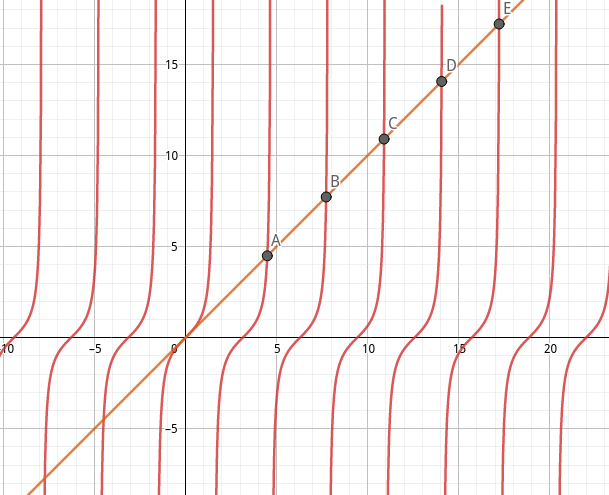
\includegraphics[width=\linewidth]{pic1.png}
			\end{figure}
			То есть $n\pi<x_n<(n+1)\pi$
			
			Тогда $\sum_{n=2}^{\infty}\frac{1}{(\pi n)^\epsilon}<\sum_{n=1}^{\infty}\frac{1}{x_n^2}<\sum_{n=1}^{\infty}\frac{1}{(\pi n)^2}$
			
			Но и левый и правый ряды очевидно сходятся, таким образом сходится и наш.
		\end{enumerate}
		
	\end{enumerate}
\end{document}